\RequirePackage[OT1]{fontenc} 
\documentclass[journal]{IEEEtran}

% *** CITATION PACKAGES ***
\usepackage[style=ieee]{biblatex} 
\bibliography{example_bib.bib}    %your file created using JabRef

% *** MATH PACKAGES ***
\usepackage{amsmath}
\usepackage{amssymb}

% Table Packages
\usepackage{booktabs}
\usepackage{tabularx}

% *** PDF, URL AND HYPERLINK PACKAGES ***
\usepackage{url}
% correct bad hyphenation here
\hyphenation{op-tical net-works semi-conduc-tor}
\usepackage{graphicx}  %needed to include png, eps figures
\graphicspath{{./images/}}
\usepackage{float}  % used to fix location of images i.e.\begin{figure}[H]

%Mathcha
\usepackage{physics}
\usepackage{amsmath}
\usepackage{tikz}
\usepackage{mathdots}
\usepackage{yhmath}
\usepackage{cancel}
\usepackage{color}
\usepackage{siunitx}
\usepackage{array}
\usepackage{multirow}
\usepackage{amssymb}
\usepackage{gensymb}
\usepackage{tabularx}
\usepackage{extarrows}
\usepackage{booktabs}
\usetikzlibrary{fadings}
\usetikzlibrary{patterns}
\usetikzlibrary{shadows.blur}
\usetikzlibrary{shapes}
\usepackage{bigfoot} % to allow verbatim in footnote
\usepackage{listings}
\usepackage[final,numbered,framed]{matlab-prettifier}
\usepackage[T1]{fontenc} 

%%% MATLAB LISTING
% \let\ph\mlplaceholder % shorter macro
% \lstMakeShortInline"

\lstset{
style = Matlab-editor, basicstyle=\mlttfamily\footnotesize,
%   escapechar         = ",
xleftmargin=3em,
xrightmargin=3em,
  mlshowsectionrules = true,
}

\newcommand{\eqdef}{\mathrel{:\mathop=}}

\begin{document}

\title{Stereo Radio Signals}
% \\ \small{EE4361 Class Project}

% author names 
\author{STEPHEN ANSEL CAMPBELL \\
    \emph{sac170630@utdallas.edu} \\
    EE 4361 --- INTRO TO DIGITAL SIGNAL PROCESSING
}

% The report headers
\markboth{EE 4361 Dr.\ Issa Panahi, \today}%do not delete next lines
{EE 4361 Dr.\ Panahi}

% make the title area
\maketitle

% As a general rule, do not put math, special symbols or citations
% in the abstract or keywords.
\begin{abstract}
    Methods to simultaneously transmit signal (mono) and dual (stereo) channel
    audio signals are valuable and important applications of signal processing.
    This report details one such method which utilizes fast analog to digital
    conversion with a digital signal processor.  By transforming our signal into
    the digital domain, this method leverages the techniques discussed and
    elaborated on in the course \emph{EE4361}  taught by Dr.\ Panahi.
\end{abstract}

\section{Introduction}

\IEEEPARstart{B}{ecause} using physical digital signal processors currently on
the market would add cost and complexity to implementing a particular method,
\emph{MATLAB} is utilized to simulate, design, and prototype a digital signal
processing pipeline that can act as a stereo receiver. This pipeline transforms
the signal received by an antenna and to a separate left channel and right
channel. The formulation of the problem is given and followed by the design of
the digital signal pipeline. Finally, an example is discussed, showing  the pipeline
indeed transforms the modulated signal is into its desired audio outputs.

\section{Formulation}

% \textbf{Develop and write down the complete analytical formulation of the
%     problem, at the transmitter and at the receiver and, how and why \(x_1(n)\) and
%     \(x_2(n)\)and the gains are obtained in your report.}


The signals start as analog voltage magnitudes with the notation given below.
\begin{gather*}
    \begin{aligned}
        x_{1,a}( t) & \eqdef \text{male speaker}   \\
        x_{2,a}( t) & \eqdef \text{female speaker}
    \end{aligned}
\end{gather*}


The signals  are then low pass filtered such that they are bandlimited to 5kHz.
This is shown with the signals' convolution with \(h_{lp,f_{c} =5\text{kHz}}(
t)\).



\begin{equation*}
    \begin{aligned}
        x_{1,\text{bandlimited}}( t) & =x_{1,a}( t) *h_{lp,f_{c} =5\text{kHz}}( t) \\
        x_{2,\text{bandlimited}}( t) & =x_{2,a}( t) *h_{lp,f_{c} =5\text{kHz}}( t)
    \end{aligned}
\end{equation*}


These resultant signals are sampled at twice their bandwidth at  \(\displaystyle
F_{s,\text{mic}} =16\times 10^{3}\text{Hz} ,\ T_{s,\text{mic}}
=1/F_{s,\text{mic}}\). The sampling is stopped after a time \(T_f\) which is
equivalent to rectangular windowing between 0 and \(\displaystyle T_{F}\).

\begin{equation*}
    \begin{aligned}
        x_{1}( n) & =x_{1,\text{bandlimited}}( t)\Bigr|_{t=nT_{s,\text{mic}}} ,\ 0< nT_{s,\text{mic}} < T_{F}    \\
        x_{2}( n) & =x_{2,\text{bandlimited}}( t) \ \Bigr|_{t=nT_{s,\text{mic}}} ,\ 0< nT_{s,\text{mic}} < T_{F}
    \end{aligned}
\end{equation*}

In the digital transmission pipeline, the signals are added and subtracted. The sum signal is the signal channel (mono) signal.
The difference signal will eventually allow the left and right channels to be separated on stereo receivers.

\begin{equation*}
    \begin{aligned}
        s_{1}( n) & =x_{1}( n) +x_{2}( n) \\
        s_{2}( n) & =x_{1}( n) -x_{2}( n)
    \end{aligned}
\end{equation*}

The signals are then digitally modulated to prepare for transmission.  This
modulation occurs at \(\displaystyle f_{\text{carrier}} =70\text{kHz}\) and
\(\displaystyle f_{\text{carrier}} +f_{\Delta } =90\text{kHz}\).


\begin{equation*}
    \begin{aligned}
                                   & 0< nT_{s,\text{mic}} < T_{F}                                                                  \\
        s_{1,\text{modulated}}( n) & =s_{1}( n)\cos\left(\frac{2\pi f_{\text{carrier}}}{F_{s,\text{mic}}} n\right) \\
        s_{2,\text{modulated}}( n) & =s_{2}( n)\cos\left(\frac{2\pi ( f_{\text{carrier}} +f_{\Delta })}{F_{s,\text{mic}}} n\right)
    \end{aligned}
\end{equation*}

The final step in the digital transmission pipeline is adding the sum and difference signals.
\begin{align*}
    TX( n) & =s_{1,\text{modulated}}( n) +s_{2,\text{modulated}}( n)
\end{align*}

The completed digital transmission signal must be converted to analog for
transmission. In this model, an ideal D/A is used.

\begin{equation*}
    \begin{aligned}
        TX( t) & =\sum _{k=-\infty }^{\infty } TX( k) \delta ( t+kT_{s}) *h_{lp,f_{c} =90\text{kHz}}( t)
    \end{aligned}
\end{equation*}

For this model, the analog transmission is assumed to be lossless.
\begin{align*}
    RX( t) & =TX( t)
\end{align*}

After transmission, the receiver will sample the signal with an analog to
digital converter with  sampling frequency and sample interval \(\displaystyle
F_{s,\text{receiver}} =400\times 10^{3}\text{Hz} ,\ T_{s,\text{receiver}}
=1/F_{s,\text{receiver}}\), respectively. Again, because the recorded signal was
finite, the signal is windowed  between 0 and \(\displaystyle T_{F}\)


\begin{align*}
    RX( n) & =RX( t)\Bigr|_{t=nT_{s,\text{receiver}}} ,\ 0< nT_{s,\text{receiver}} < T_{F} \
\end{align*}

We now come to the main focus of the design. This received discrete time signal must be transformed
to output reconstructed versions of the left channel and right channel. For now, this is shown with
a black box function \(\operatorname{RECV}\)

\begin{align*}
    \operatorname{RECV}                  & \eqdef \text{Receiver to be designed}    \\
    \tilde{x}_{1}( n) ,\tilde{x}_{2}( n) & =\operatorname{RECV}\left( RX( n)\right)
\end{align*}

By reconstructing the original signals, the signal processing pipeline is complete.

\section{Design}

The \(\displaystyle \operatorname{RECV}\) operation is given as the below signal
processing pipeline. The pipeline goes through stages of demodulation,
filtering, addition/subtraction, and gain.

\subsection{Demodulation}

The signals of importance lie in the frequency domain at 70kHz and 90kHz. In
order to extract the signal information at those frequencies, the received signal needs to be
demodulated at both 70kHz and 90kHz. The \emph{MATLAB} implementation is shown in Fig.\ \ref{fig:demod_m}.



\begin{align*}
                                       & \ 0< nT_{s,\text{receiver}} < T_{F}                                                             \\
    RX_{\text{demodulated, 70kHz}}( n) & =RX( n)\cos\left(\frac{2\pi f_{\text{carrier}}}{F_{s,\text{receiver}}} n\right)                 \\
    RX_{\text{demodulated, 90kHz}}( n) & =RX( n)\cos\left(\frac{2\pi ( f_{\text{carrier}} +f_{\Delta })}{F_{s,\text{receiver}}} n\right)
\end{align*}


\subsection{Filtering}

Unfortunately, demodulation also results in frequency shifted replicas of the
original received signals appearing in the resultant signals. These replicas can
be removed via filtering.  Because the information signal was originally
bandlimited to 5kHz, to reconstruct the signals faithfully the demodulated
signal was also be low pass filtered to that frequency. The \emph{MATLAB}
implementation of this filtering is show in Fig.\ \ref{fig:filter_m}.

\begin{align*}
    N                 & \eqdef \operatorname{length}\left(\tilde{s}_{1}( n)\right)                                                \\
    \tilde{s}_{1}( n) & =RX_{\text{demodulated, 70kHz}}( n) \ \tikz[baseline=(char.base)]{\node[ellipse,draw] (char) {\text{N}};}
    \ h_{lp,f_{c} =5\text{kHz}}( n)                                                                                               \\
    \tilde{s}_{2}( n) & =RX_{\text{demodulated, 90kHz}}( n) \ \tikz[baseline=(char.base)]{\node[ellipse,draw] (char) {\text{N}};}
    \ _{lp,f_{c} =5\text{kHz}}( n)
\end{align*}


\subsection{Addition/Subtraction and Gain}

With the sum and difference signals now reconstructed, the left and right channels can be acquired.
Both gains must be \(\frac{1}{2}\) because each

\begin{align*}
    \tilde{x}_{1}( n) & =G_{1}\left(\tilde{s}_{1}( n) +\tilde{s}_{2}( n)\right) \\
    \tilde{x}_{2}( n) & =G_{2}\left(\tilde{s}_{1}( n) -\tilde{s}_{2}( n)\right) \\
    G_{1} ,G_{2}      & \rightarrow \frac{1}{2}
\end{align*}

\section{Results}

The example data file distributed through email is transformed and used as an
example of the functional stereo receiver digital signal processing pipeline.
The data file was analyzed the resulting signals \(x_1(n)\) and \(x_2(n)\) were
plotted in Fig.\ \ref{fig:time_recon}.  Additionally, their respective spectrums
as given by the DFT were calculated and plotted in Fig.\ \ref{fig:freq_recon}.
The right, female channel says ``The clothes dried on a thin wooden rack.~'' While the
left, male speakers says, ``The birch canoe slid on the smooth planks.~''



\begin{figure}[H]
    \begin{center}
        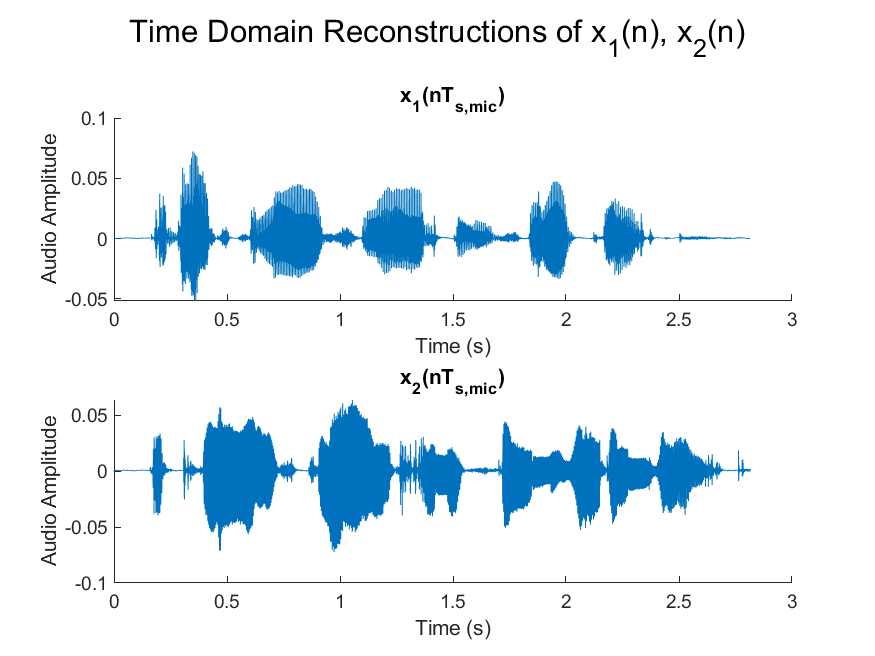
\includegraphics[width=0.4\textwidth]{time_recon.png}
        \caption{\label{fig:time_recon} Time Domain Representation of Reconstructed Signals \(x_1(n)\) and \(x_2(n)\)}
    \end{center}
\end{figure}

\begin{figure}[H]
    \begin{center}
        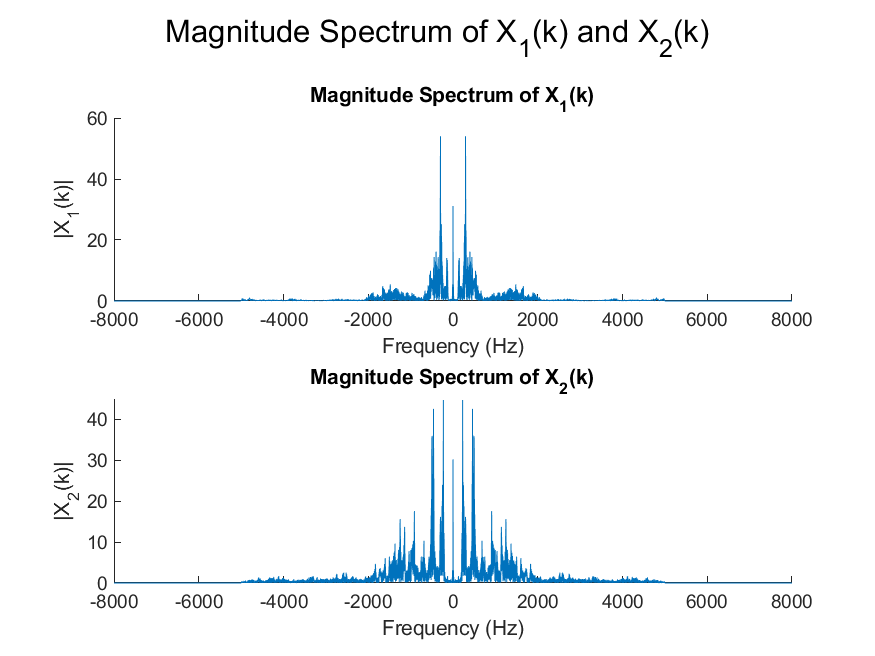
\includegraphics[width=0.4\textwidth]{freq_recon.png}
        \caption{\label{fig:freq_recon}Magnitude of DFT of Reconstructed Signals \(x_1(n)\) and \(x_2(n)\)}
    \end{center}
\end{figure}


\section{Discussion and Conclusion}

Through the discussion of this emphatically digital method to transmit and
receive both mono and stereo audio, immense familiarity has been gained with the
fundamentals of  digital signal processing.

\appendices
\section{\emph{MATLAB} Implementations}

\begin{figure}[h]
    \caption{\label{fig:filter_m} \emph{MATLAB} Implementation of Filtering}
    \begin{lstlisting}
function filtered_sig = ideal_lowpass(signal_fft,cutoff_freq,Fs)
    num_samples = length(signal_fft);
    passband_freq_index = floor(cutoff_freq*num_samples/Fs)
    rectangle = zeros(size(signal_fft));
    rectangle(1:passband_freq_index+1) = 1;
    rectangle(end-passband_freq_index+1:end) = 1;
    filtered_sig = rectangle .* signal_fft;
end
\end{lstlisting}
\end{figure}

\begin{figure}[h]
    \caption{\label{fig:demod_m} \emph{MATLAB} Implementation of Demodulation}
    \begin{center}
        \begin{lstlisting}
function demodsig = demodulate_signal(time_sig, shift_down_freq, Fs) 
    num_samples = length(time_sig);
    carrier = cos(2*pi*shift_down_freq*(0:num_samples-1)/Fs)'
    demod_time_sig = time_sig .* carrier;
    demodsig = demod_time_sig
end
\end{lstlisting}


    \end{center}
\end{figure}

\section{Repository}
This source of the latex report, the \emph{MATLAB} code, and all references can
be found at \url{https://github.com/Stephen-Campbell-UTD/DSP_Project}

\end{document}